% =====================================================================
%  GloVe: Architecture & Internals
%  A guided tour of the Stanford GloVe reference implementation.
%  Build:  latexmk -pdf glove_architecture.tex
% =====================================================================
\documentclass[11pt,a4paper]{article}

\usepackage[T1]{fontenc}
\usepackage[utf8]{inputenc}
\usepackage{lmodern}
\usepackage{inconsolata}
\usepackage[margin=2.5cm]{geometry}
\usepackage{microtype}
\usepackage{amsmath,amssymb,mathtools}
\usepackage{booktabs,tabularx,array}
\usepackage{enumitem}
\usepackage{xcolor}
\usepackage{listings}
\usepackage{tikz}
\usetikzlibrary{arrows.meta,positioning,shapes.geometric,shapes.multipart,shapes.symbols,calc,fit,backgrounds,decorations.pathreplacing,patterns}
\usepackage{pgfplots}
\pgfplotsset{compat=1.18}
\usepackage[most]{tcolorbox}
\usepackage{fancyhdr}
\usepackage[colorlinks=true,linkcolor=blue!50!black,urlcolor=blue!50!black,citecolor=blue!50!black]{hyperref}

% ---------------------------------------------------------------------
%  Styling
% ---------------------------------------------------------------------
\definecolor{codebg}{HTML}{F6F8FA}
\definecolor{codeframe}{HTML}{D0D7DE}
\definecolor{kw}{HTML}{0550AE}
\definecolor{cm}{HTML}{6E7781}
\definecolor{st}{HTML}{0A3069}
\definecolor{stageA}{HTML}{DDF4FF}
\definecolor{stageB}{HTML}{FFF8C5}
\definecolor{stageC}{HTML}{FBEFFF}
\definecolor{stageD}{HTML}{DAFBE1}
\definecolor{fileC}{HTML}{F6F8FA}

\lstdefinestyle{c}{
  language=C,
  basicstyle=\ttfamily\small,
  keywordstyle=\color{kw}\bfseries,
  commentstyle=\color{cm},
  stringstyle=\color{st},
  backgroundcolor=\color{codebg},
  frame=single, rulecolor=\color{codeframe},
  numbers=left, numberstyle=\tiny\color{cm}, numbersep=6pt,
  breaklines=true, columns=fullflexible, keepspaces=true,
  showstringspaces=false, xleftmargin=1.5em, framexleftmargin=1.5em,
  tabsize=4
}
\lstdefinestyle{sh}{
  language=bash,
  basicstyle=\ttfamily\small,
  backgroundcolor=\color{codebg},
  frame=single, rulecolor=\color{codeframe},
  breaklines=true, columns=fullflexible, keepspaces=true,
  showstringspaces=false
}
\lstset{style=c}

\newtcolorbox{insight}[1][]{colback=blue!3,colframe=blue!45!black,
  fonttitle=\bfseries,title={Key insight},#1}
\newtcolorbox{pitfall}[1][]{colback=red!3,colframe=red!55!black,
  fonttitle=\bfseries,title={Gotcha},#1}
\newtcolorbox{codeloc}[1][]{colback=green!3,colframe=green!40!black,
  fonttitle=\bfseries,title={Where in the code},#1}

\newcommand{\file}[1]{\texttt{#1}}
\newcommand{\fn}[1]{\texttt{#1()}}
\newcommand{\opt}[1]{\texttt{-#1}}
\newcommand{\R}{\mathbb{R}}
\newcommand{\wv}{\mathbf{w}}
\newcommand{\cv}{\tilde{\mathbf{w}}}

\pagestyle{fancy}
\fancyhf{}
\lhead{\small GloVe --- Architecture \& Internals}
\rhead{\small\thepage}
\setlength{\headheight}{14pt}

\title{\textbf{GloVe: Global Vectors for Word Representation}\\[4pt]
  \large Architecture \& Internals of the Stanford Reference Implementation}
\author{Companion document for the \texttt{stanfordnlp/GloVe} source tree}
\date{\today}

\begin{document}
\maketitle

\begin{abstract}
\noindent
This document explains GloVe (Global Vectors for Word Representation) end to end, from the mathematical model to the bytes on disk.
Part~I covers the \emph{why}: the idea that ratios of co-occurrence probabilities encode
meaning, and how that idea becomes a weighted least-squares objective. Part~II covers the
\emph{how}: the four-stage C pipeline (\texttt{vocab\_count} $\rightarrow$ \texttt{cooccur}
$\rightarrow$ \texttt{shuffle} $\rightarrow$ \texttt{glove}), the data structures and file
formats that connect the stages, the memory-management heuristics, and the lock-free
multi-threaded AdaGrad (adaptive gradient) trainer. Part~III covers operations: hyper-parameters, resource
sizing, evaluation, reproducibility, and known quirks found while reading the code.
Each section points to the functions in \file{src/} that implement it, so you can read the
document and the code side by side.
\end{abstract}

\tableofcontents
\newpage

% =====================================================================
\part{The Model}
% =====================================================================

\section{The problem GloVe solves}

A \emph{word embedding} maps each vocabulary word $i$ to a dense vector $\wv_i\in\R^d$
(typically $d\in\{50,100,200,300\}$) so that geometric relationships between vectors
mirror semantic and syntactic relationships between words. The classic demonstration is
analogy arithmetic:
\[
  \wv_{\text{king}} - \wv_{\text{man}} + \wv_{\text{woman}} \;\approx\; \wv_{\text{queen}}.
\]

Before GloVe there were two main families of methods:

\begin{description}[leftmargin=1.5em]
  \item[Global matrix factorisation] Latent Semantic Analysis (LSA), Hyperspace Analogue to Language (HAL), and positive pointwise mutual information (PPMI) followed by singular value decomposition (SVD). Build a large word--context
    count matrix over the whole corpus and factorise it. These use corpus-wide statistics
    efficiently, but they do poorly on analogy tasks because raw or log counts are
    dominated by frequent words and SVD weights every cell the same.
  \item[Local context-window prediction] (word2vec's skip-gram and continuous bag-of-words (CBOW) models). Slide a window over
    the text and train a classifier to predict context words. These produce good linear
    structure, but they scan the corpus window by window and never use the aggregate
    counts directly, so repeated co-occurrences are processed again each time they appear.
\end{description}

GloVe (Pennington, Socher \& Manning, Conference on Empirical Methods in Natural Language Processing (EMNLP) 2014) combines the two. It \textbf{collects
global co-occurrence counts once}, then \textbf{fits a log-bilinear regression model} to
the non-zero counts. This gives word2vec-style linear structure at the cost of
\emph{factorising a matrix}: training scales with the number of non-zero entries of the
co-occurrence matrix, not with corpus length.

\section{Notation and abbreviations}

\begin{center}
\begin{tabularx}{\linewidth}{>{$}l<{$}X}
\toprule
\text{Symbol} & Meaning \\
\midrule
V & Vocabulary size (number of lines in \file{vocab.txt}). \\
d & Vector dimension (\opt{vector-size}). \\
X \in \R^{V\times V} & Co-occurrence matrix. $X_{ij}$ is the (distance-weighted) number of
  times word $j$ appears in the context of word $i$. \\
X_i = \sum_k X_{ik} & Total context mass of word $i$. \\
P_{ij} = X_{ij}/X_i & Probability that $j$ appears in the context of $i$. \\
\wv_i,\ \cv_j \in \R^d & \emph{Word} vector of $i$ and \emph{context} vector of $j$
  (two separate parameter sets). \\
b_i,\ \tilde b_j \in \R & Word and context biases. \\
f(\cdot) & Weighting function, with parameters $x_{\max}$ (\opt{x-max}) and $\alpha$ (\opt{alpha}). \\
\mathrm{nnz}(X) & Number of non-zero entries of $X$. \\
\bottomrule
\end{tabularx}
\end{center}

\subsection*{Abbreviations}
Each abbreviation is also spelled out where it first appears in the text.
\begin{center}
\small
\begin{tabularx}{\linewidth}{@{}l>{\raggedright\arraybackslash}X@{\hspace{1.5em}}l>{\raggedright\arraybackslash}X@{}}
\toprule
AdaGrad & Adaptive gradient (optimiser) & NaN & Not a number \\
CBOW & Continuous bag-of-words (word2vec model) & NeurIPS & Neural Information Processing Systems (conference) \\
CREC & Co-occurrence record (C struct) & nnz & Number of non-zero entries \\
EMNLP & Empirical Methods in Natural Language Processing (conference) & PMI & Pointwise mutual information \\
EOF & End of file & PPMI & Positive pointwise mutual information \\
GB & Gigabyte ($2^{30}$ bytes in the code) & pthreads & POSIX threads \\
GloVe & Global Vectors for Word Representation & PTB & Penn Treebank \\
HAL & Hyperspace Analogue to Language & RAM & Random-access memory \\
HASHREC & Hash-table record (C struct) & SGD & Stochastic gradient descent \\
I/O & Input/output & SSD & Solid-state drive \\
JMLR & Journal of Machine Learning Research & stdin, stdout, stderr & Standard input, output, error \\
LSA & Latent Semantic Analysis & SVD & Singular value decomposition \\
TSIZE & Hash-table size (constant) & UTF-8 & Unicode Transformation Format, 8-bit \\
\bottomrule
\end{tabularx}
\end{center}

\section{From probability ratios to a loss function}

\subsection{The core observation}

Take two related words, $i=\text{ice}$ and $j=\text{steam}$, and ask how probe words $k$
co-occur with each of them. The paper reports (6-billion-token corpus):

\begin{center}
\begin{tabular}{lcccc}
\toprule
Probe $k$ & solid & gas & water & fashion \\
\midrule
$P(k\mid\text{ice})$   & $1.9\times10^{-4}$ & $6.6\times10^{-5}$ & $3.0\times10^{-3}$ & $1.7\times10^{-5}$\\
$P(k\mid\text{steam})$ & $2.2\times10^{-5}$ & $7.8\times10^{-4}$ & $2.2\times10^{-3}$ & $1.8\times10^{-5}$\\
\midrule
Ratio & $\mathbf{8.9}$ & $\mathbf{8.5\times10^{-2}}$ & $1.36$ & $0.96$\\
\bottomrule
\end{tabular}
\end{center}

The raw probabilities are hard to read. The \emph{ratio} $P_{ik}/P_{jk}$ is clear: it is
large for words specific to ice (\emph{solid}), small for words specific to steam
(\emph{gas}), and close to 1 for words related to both (\emph{water}) or to neither
(\emph{fashion}). \textbf{Meaning is carried by ratios of co-occurrence probabilities.}

\subsection{Deriving the model}

We want a function $F$ with
\begin{equation}
  F(\wv_i, \wv_j, \cv_k) = \frac{P_{ik}}{P_{jk}}.
\end{equation}
Three requirements narrow it down:

\begin{enumerate}
  \item \textbf{Vector spaces are linear}, so we compare $i$ and $j$ through their difference:
        $F(\wv_i-\wv_j,\cv_k)$.
  \item \textbf{The right-hand side is a scalar}, so we reduce the arguments with a dot
        product: $F\big((\wv_i-\wv_j)^\top\cv_k\big)$. This keeps the dimensions from mixing in
        arbitrary ways.
  \item \textbf{Word and context roles are interchangeable} ($X$ is symmetric for a
        symmetric window), so $F$ should turn differences into ratios. That makes it a
        homomorphism from $(\R,+)$ to $(\R_{>0},\times)$:
        \[
          F\big((\wv_i-\wv_j)^\top\cv_k\big) = \frac{F(\wv_i^\top\cv_k)}{F(\wv_j^\top\cv_k)},
        \]
        whose solution is $F=\exp$.
\end{enumerate}

Hence $\exp(\wv_i^\top\cv_k)=P_{ik}=X_{ik}/X_i$, i.e.
\[
  \wv_i^\top\cv_k = \log X_{ik} - \log X_i.
\]
The term $\log X_i$ does not depend on $k$, so it is absorbed into a bias $b_i$. A context
bias $\tilde b_k$ restores the symmetry:
\begin{equation}
  \boxed{\;\wv_i^\top\cv_k + b_i + \tilde b_k \;=\; \log X_{ik}\;}
  \label{eq:model}
\end{equation}

\subsection{The weighted least-squares objective}

Equation~\eqref{eq:model} cannot hold exactly, so we fit it by least squares. Two problems
remain: $\log 0$ is undefined, and rare co-occurrences are noisy while very frequent ones
(\emph{the}, \emph{of}) should not dominate. GloVe adds a weight $f(X_{ij})$ to each term:
\begin{equation}
  J \;=\; \sum_{i,j\,:\,X_{ij}>0} f(X_{ij})\,\Big(\wv_i^\top\cv_j + b_i + \tilde b_j - \log X_{ij}\Big)^2
  \label{eq:loss}
\end{equation}
\begin{equation}
  f(x) = \begin{cases} (x/x_{\max})^{\alpha} & x < x_{\max}\\ 1 & \text{otherwise}\end{cases}
  \label{eq:weight}
\end{equation}

The sum runs only over \textbf{non-zero} cells. That is why the pipeline only ever stores
sparse $(i,j,X_{ij})$ triples. It also requires $f(0)=0$, so zero cells contribute nothing.

\begin{figure}[h]
\centering
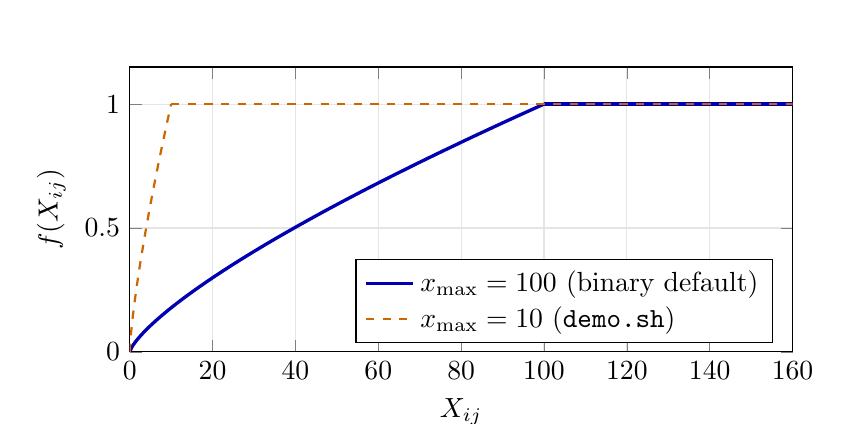
\begin{tikzpicture}
\begin{axis}[width=10cm,height=5.2cm,xlabel={$X_{ij}$},ylabel={$f(X_{ij})$},
  xmin=0,xmax=160,ymin=0,ymax=1.15,grid=major,grid style={gray!20},
  legend pos=south east,legend cell align=left]
  \addplot[very thick,blue!70!black,domain=0:100,samples=200]{(x/100)^0.75};
  \addplot[very thick,blue!70!black,domain=100:160,forget plot]{1};
  \addplot[thick,dashed,orange!80!black,domain=0:10,samples=100]{(x/10)^0.75};
  \addplot[thick,dashed,orange!80!black,domain=10:160,forget plot]{1};
  \legend{$x_{\max}=100$ (binary default), $x_{\max}=10$ (\file{demo.sh})}
\end{axis}
\end{tikzpicture}
\caption{The weighting function with $\alpha=0.75$. Rare pairs are down-weighted and
frequent pairs are capped at weight 1.}
\end{figure}

\begin{insight}
\begin{itemize}[leftmargin=1em,nosep]
  \item $\alpha=3/4$ is the same exponent word2vec uses for its negative-sampling
        distribution. Empirically it beats $\alpha=1$.
  \item $x_{\max}$ should match corpus scale. The binary's default is 100 (the paper's
        value for multi-billion-token corpora). \file{demo.sh} and \file{Training\_README.md}
        use 10.
  \item GloVe learns \emph{two} embedding tables, $W$ and $\tilde W$. With a symmetric
        context they are equivalent up to random initialisation, so the default output is
        their sum $\wv_i+\cv_i$, which acts as a small ensemble and usually scores a little
        better.
\end{itemize}
\end{insight}

\subsection{Gradients}

Write $\delta_{ij} = \wv_i^\top\cv_j + b_i + \tilde b_j - \log X_{ij}$ (the code calls this
\texttt{diff}) and $g_{ij}=f(X_{ij})\,\delta_{ij}$ (the code's \texttt{fdiff}). For a single
term of $\tfrac12 J$:
\begin{align}
  \nabla_{\wv_i} &= g_{ij}\,\cv_j, &
  \nabla_{\cv_j} &= g_{ij}\,\wv_i, &
  \partial_{b_i} &= \partial_{\tilde b_j} = g_{ij}.
\end{align}
The implementation reports the cost as $\tfrac12 f\delta^2$, so the factor 2 drops out.

\subsection{Relationship to other models}

The paper shows that skip-gram's objective, summed over the corpus, can be written as
$-\sum_{i,j} X_{ij}\log Q_{ij}$, a weighted cross-entropy between the empirical $P$ and the
softmax model $Q$. GloVe replaces (a) cross-entropy with squared error on log counts,
which avoids the softmax normalisation, and (b) the implicit weight $X_{ij}$ with the
bounded weight $f(X_{ij})$. In this sense GloVe is a weighted, log-count matrix
factorisation that is trained by stochastic gradient descent (SGD).

% =====================================================================
\part{The Implementation}
% =====================================================================

\section{Repository map}

\begin{center}
\begin{tabularx}{\linewidth}{lrX}
\toprule
Path & Lines & Role \\
\midrule
\file{src/common.\{h,c\}} & 217 & Shared types (\texttt{CREC}, the co-occurrence record; \texttt{HASHREC}, the hash-table record), the hash
  function, the tokenizer \fn{get\_word}, command-line parsing \fn{find\_arg}. \\
\file{src/vocab\_count.c} & 172 & Stage 1: unigram counts $\rightarrow$ \file{vocab.txt}. \\
\file{src/cooccur.c}      & 445 & Stage 2: windowed co-occurrence counting with a hybrid
  dense/sparse store and external merge sort $\rightarrow$ \file{cooccurrence.bin}. \\
\file{src/shuffle.c}      & 210 & Stage 3: out-of-core shuffle $\rightarrow$
  \file{cooccurrence.shuf.bin}. \\
\file{src/glove.c}        & 559 & Stage 4: multi-threaded AdaGrad training $\rightarrow$
  \file{vectors.\{txt,bin\}}. \\
\file{Makefile}           & 48  & Builds four executables in \file{build/}. \\
\file{demo.sh}            & 57  & End-to-end run on \texttt{text8} plus evaluation. \\
\file{randomization.test.sh} & -- & Determinism tests (seeds, checkpoint/resume). \\
\file{eval/python/}       & -- & Analogy evaluation, nearest neighbours, interactive analogies. \\
\file{eval/\{matlab,octave\}/} & -- & Same evaluation for MATLAB/Octave. \\
\file{eval/question-data/} & -- & The Google analogy test set (14 files). \\
\bottomrule
\end{tabularx}
\end{center}

The system is \textbf{four independent Unix filters} connected by files, with no shared
state beyond those files. Each tool reads standard input (\texttt{stdin}) and/or named files, writes its
result to standard output (\texttt{stdout}) or named files, and writes logs to standard
error (\texttt{stderr}). This keeps
each stage simple, lets you re-run any stage alone (for example, retrain with a new $d$
without recounting), and lets every stage except the trainer work out of core.

\section{The pipeline at a glance}

\begin{figure}[h]
\centering
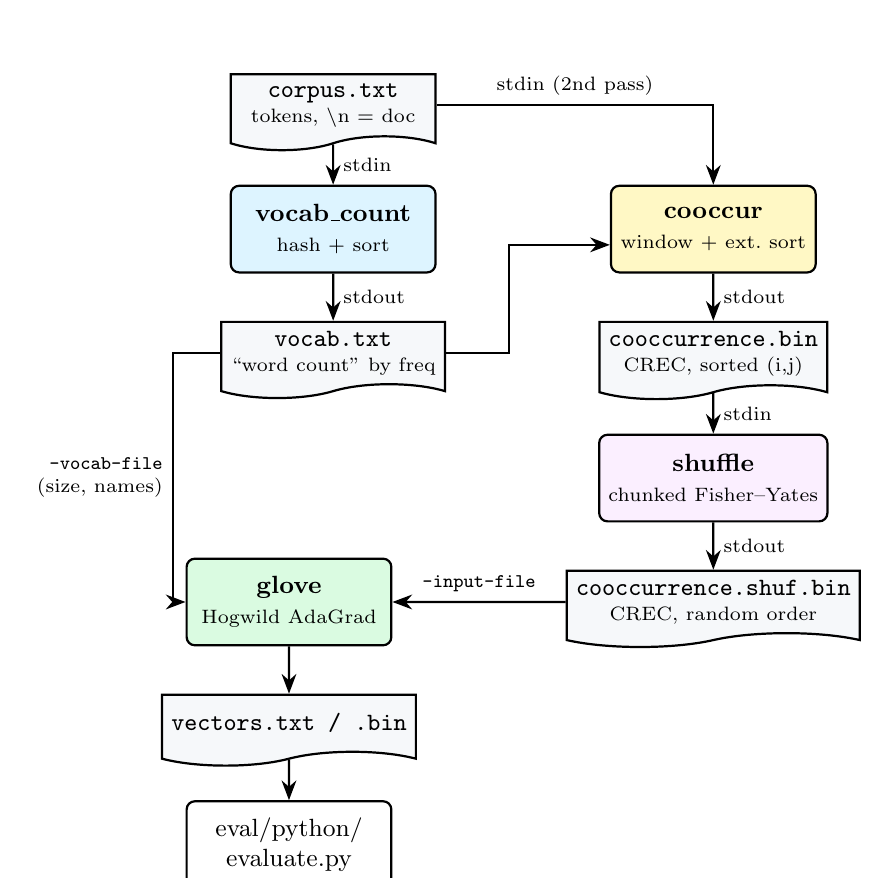
\begin{tikzpicture}[
  node distance=6mm and 6mm,
  tool/.style={draw,rounded corners=3pt,thick,minimum width=26mm,minimum height=11mm,align=center,font=\small},
  data/.style={draw,shape=tape,tape bend top=none,thick,fill=fileC,minimum width=26mm,minimum height=9mm,align=center,font=\small\ttfamily},
  arr/.style={-{Stealth[length=2.5mm]},thick}
]
\node[data] (corpus) {corpus.txt\\[-2pt]{\scriptsize\rmfamily tokens, \textbackslash n = doc}};
\node[tool,fill=stageA,below=of corpus] (vc) {\textbf{vocab\_count}\\{\scriptsize hash + sort}};
\node[data,below=of vc] (vocab) {vocab.txt\\[-2pt]{\scriptsize\rmfamily ``word count'' by freq}};
\node[tool,fill=stageB,right=22mm of vc] (co) {\textbf{cooccur}\\{\scriptsize window + ext.\ sort}};
\node[data,below=of co] (cbin) {cooccurrence.bin\\[-2pt]{\scriptsize\rmfamily CREC, sorted (i,j)}};
\node[tool,fill=stageC,below=of cbin] (sh) {\textbf{shuffle}\\{\scriptsize chunked Fisher--Yates}};
\node[data,below=of sh] (sbin) {cooccurrence.shuf.bin\\[-2pt]{\scriptsize\rmfamily CREC, random order}};
\node[tool,fill=stageD,left=22mm of sbin] (gl) {\textbf{glove}\\{\scriptsize Hogwild AdaGrad}};
\node[data,below=of gl] (vec) {vectors.txt / .bin};
\node[tool,below=of vec] (ev) {eval/python/\\evaluate.py};

\draw[arr] (corpus) -- node[right,font=\scriptsize]{stdin} (vc);
\draw[arr] (vc) -- node[right,font=\scriptsize]{stdout} (vocab);
\draw[arr] (corpus.east) -| node[pos=0.25,above,font=\scriptsize]{stdin (2nd pass)} (co.north);
\draw[arr] (vocab.east) -- ++(8mm,0) |- ($(co.west)+(0,-2mm)$);
\draw[arr] (co) -- node[right,font=\scriptsize]{stdout} (cbin);
\draw[arr] (cbin) -- node[right,font=\scriptsize]{stdin} (sh);
\draw[arr] (sh) -- node[right,font=\scriptsize]{stdout} (sbin);
\draw[arr] (sbin) -- node[above,font=\scriptsize]{\opt{input-file}} (gl);
\draw[arr] (vocab.west) -- ++(-6mm,0) |- node[pos=0.25,left,font=\scriptsize,align=right]{\opt{vocab-file}\\(size, names)} (gl.west);
\draw[arr] (gl) -- (vec);
\draw[arr] (vec) -- (ev);
\end{tikzpicture}
\caption{Data flow. The corpus is read twice, once for unigrams and once for co-occurrences.
Everything after \texttt{cooccur} works on a compact binary list of non-zero cells.}
\label{fig:pipeline}
\end{figure}

\begin{lstlisting}[style=sh,caption={The canonical invocation (from \file{demo.sh}).}]
build/vocab_count -min-count 5 -verbose 2                 < text8 > vocab.txt
build/cooccur -memory 4.0 -vocab-file vocab.txt -window-size 15 < text8 > cooccurrence.bin
build/shuffle -memory 4.0                       < cooccurrence.bin > cooccurrence.shuf.bin
build/glove -save-file vectors -threads 8 -input-file cooccurrence.shuf.bin \
            -x-max 10 -iter 15 -vector-size 50 -binary 2 -vocab-file vocab.txt
\end{lstlisting}

\section{Shared foundations: \file{common.c}}

\subsection{The universal record: \texttt{CREC}}

\begin{lstlisting}
typedef double real;
typedef struct cooccur_rec { int word1; int word2; real val; } CREC;   // 4+4+8 = 16 bytes
\end{lstlisting}

Every binary file between stages 2, 3 and 4 is a headerless array of \texttt{CREC}s written
with \fn{fwrite}. Consequences:
\begin{itemize}[nosep]
  \item File size $= 16\times\text{nnz}(X)$ bytes, and the record count is
        \texttt{filesize/16} (this is how \fn{train\_glove} sizes its work).
  \item Word ids are \textbf{1-based frequency ranks}: id 1 is the most frequent word,
        which is line 1 of \file{vocab.txt}.
  \item The format is native-endian and native-layout, so it is not portable across
        architectures with different endianness or padding.
\end{itemize}

\subsection{Tokenisation contract: \fn{get\_word}}

The tools do no linguistic processing. The corpus must already be tokenised and, if you
want it, lowercased (\file{Training\_README.md} uses the Stanford Penn Treebank (PTB) tokenizer with
\texttt{-lowerCase}). \fn{get\_word} follows these rules:
\begin{itemize}[nosep]
  \item Tokens are separated by spaces, tabs, or newlines. \texttt{\textbackslash r} is ignored.
  \item \textbf{A newline marks a document boundary}. The function returns 1 for a newline
        or end of file (EOF) on its own, and \texttt{cooccur} then resets its window, so context never
        crosses lines.
  \item Tokens longer than 999 bytes are truncated, with care not to split a multi-byte
        UTF-8 (Unicode Transformation Format, 8-bit) sequence.
\end{itemize}

\subsection{Hash table}

A fixed array of $\texttt{TSIZE}=2^{20}$ buckets (\texttt{TSIZE} = table size) with separate chaining, a cheap
shift-xor string hash (\fn{bitwisehash}, by Hugh Williams), and
\textbf{move-to-front on access}. Word frequencies follow Zipf's law, so a few words
account for most lookups. Moving a found record to the head of its chain makes those
lookups close to $O(1)$ even when chains get long for large vocabularies.

\section{Stage 1 --- \texttt{vocab\_count}}

\begin{codeloc}
\file{src/vocab\_count.c}: \fn{hashinsert}, \fn{get\_counts}, \fn{CompareVocab},
\fn{CompareVocabTie}.
\end{codeloc}

\paragraph{Algorithm.}
\begin{enumerate}[nosep]
  \item Stream tokens from \texttt{stdin} into the hash table, incrementing counts. The
        literal token \texttt{<unk>} is rejected because it is reserved for the output.
  \item Copy all hash records into an array.
  \item If \opt{max-vocab}~$N$ is set and exceeded, first sort by count \emph{without} a
        tie-break. Words with equal counts then end up in a pseudo-random order, so
        truncation at $N$ does not favour the start of the alphabet.
  \item Sort the first $N$ by (count desc, word asc).
  \item Print \texttt{word count} lines, stopping at the first count below \opt{min-count}.
\end{enumerate}

\paragraph{Output contract.} Line $r$ of \file{vocab.txt} is the word with id $r$.
Every later stage relies on this: \texttt{cooccur} assigns ids by line number, and
\texttt{glove} counts lines to get $V$ and re-reads the file to name output rows.
\textbf{Never edit \file{vocab.txt} between stages.}

\section{Stage 2 --- \texttt{cooccur}}

\begin{codeloc}
\file{src/cooccur.c}: \fn{get\_cooccurrence} (counting), \fn{write\_chunk},
\fn{merge\_files} (k-way merge), \fn{insert}/\fn{delete} (binary heap), and the
memory heuristic in \fn{main}.
\end{codeloc}

This is the most heavily engineered stage. For a corpus of billions of tokens, $X$ has
$V^2$ cells ($\sim10^{11}$ for $V=400$k) but only billions of non-zeros, and their
distribution is very skewed.

\subsection{Windowed counting}

The tool keeps a circular buffer \texttt{history[window\_size]} of the ids of the previous
in-vocabulary tokens on the current line. For each new in-vocabulary target $w_2$ at
position $j$, it visits each left-context word $w_1$ at position $k\in[j-W, j-1]$ and adds
\[
  \text{increment} = \begin{cases}1/(j-k) & \text{\opt{distance-weighting} 1 (default)}\\ 1 & \text{otherwise}\end{cases}
\]
to $X_{w_1 w_2}$. With \opt{symmetric}~1 (the default) it also adds the same amount to
$X_{w_2 w_1}$. That is how right context is counted without ever looking ahead.

\begin{pitfall}
Out-of-vocabulary tokens are \emph{skipped entirely}: they are not added to
\texttt{history} and they do not advance the position $j$. Distances are therefore
measured in \emph{in-vocabulary} tokens, and a high \opt{min-count} makes the effective
window span more raw text.
\end{pitfall}

\paragraph{Worked example.} Corpus line \texttt{the cat sat on the mat}, window $W=2$,
symmetric, distance-weighted. Vocabulary ids: the=1, then ties sorted alphabetically:
cat=2, mat=3, on=4, sat=5.

\begin{center}
\begin{tabular}{clll}
\toprule
$j$ & target & left context (distance) & increments (both directions)\\
\midrule
1 & cat & the (1) & $X_{\text{the,cat}}\mathrel{+}=1$ \\
2 & sat & cat (1), the (2) & $X_{\text{cat,sat}}\mathrel{+}=1,\ X_{\text{the,sat}}\mathrel{+}=\tfrac12$ \\
3 & on  & sat (1), cat (2) & $X_{\text{sat,on}}\mathrel{+}=1,\ X_{\text{cat,on}}\mathrel{+}=\tfrac12$ \\
4 & the & on (1), sat (2)  & $X_{\text{on,the}}\mathrel{+}=1,\ X_{\text{sat,the}}\mathrel{+}=\tfrac12$ \\
5 & mat & the (1), on (2)  & $X_{\text{the,mat}}\mathrel{+}=1,\ X_{\text{on,mat}}\mathrel{+}=\tfrac12$ \\
\bottomrule
\end{tabular}
\end{center}
Result: $X_{\text{the,sat}}=1.0$ (two half-weight hits), $X_{\text{the,cat}}=X_{\text{cat,sat}}
=X_{\text{sat,on}}=X_{\text{on,the}}=X_{\text{the,mat}}=1$, $X_{\text{cat,on}}=X_{\text{on,mat}}=0.5$,
and the transposes have the same values. Sixteen non-zero \texttt{CREC}s are emitted.

\subsection{Hybrid dense/sparse storage}

The key design decision follows from Zipf's law: if words are ranked by frequency, the
count of the word with rank $r$ is roughly proportional to $1/r$, so the expected
co-occurrence count of $(a,b)$ falls off roughly like $1/(ab)$. Pairs with a
\textbf{small rank product} are therefore dense and hot, and pairs with a large product are
sparse.

\begin{figure}[h]
\centering
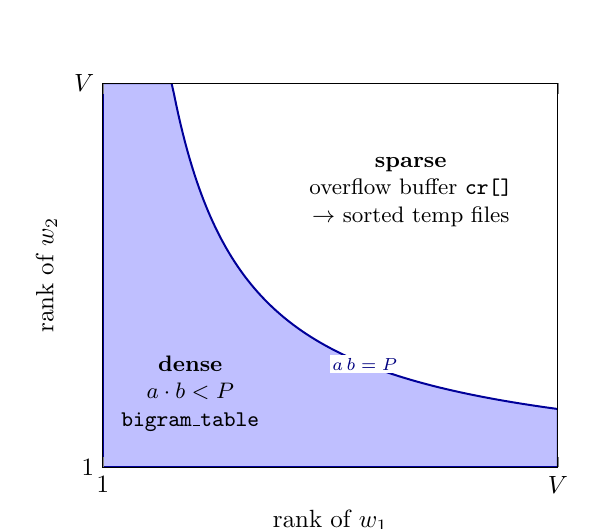
\begin{tikzpicture}[scale=0.9]
\begin{axis}[width=8cm,height=7cm,xmin=1,xmax=100,ymin=1,ymax=100,
  xlabel={rank of $w_1$},ylabel={rank of $w_2$},axis on top,
  xtick={1,100},xticklabels={1,$V$},ytick={1,100},yticklabels={1,$V$}]
  \addplot[fill=blue!25,draw=blue!60!black,thick,domain=1:100,samples=200]
     {min(100,1600/x)} \closedcycle;
  \node[font=\small,align=center] at (axis cs:20,20) {\textbf{dense}\\$a\cdot b<P$\\\texttt{bigram\_table}};
  \node[font=\small,align=center] at (axis cs:68,72) {\textbf{sparse}\\overflow buffer \texttt{cr[]}\\$\rightarrow$ sorted temp files};
  \node[font=\scriptsize,blue!50!black,fill=white,inner sep=1pt] at (axis cs:58,27.6) {$a\,b=P$};
\end{axis}
\end{tikzpicture}
\caption{Partition of the $V\times V$ matrix by rank product. The region under the
hyperbola $a\,b<P$ (\texttt{max\_product}) is stored in a ragged dense array and updated
in place. Everything else is appended to an in-memory overflow list.}
\label{fig:hyperbola}
\end{figure}

\paragraph{Dense part (\texttt{bigram\_table}).} A ragged 2-D array. Row $a$ has
$\min(\lfloor P/a\rfloor, V)$ columns. A prefix-sum table \texttt{lookup} gives the start
of each row:
\begin{lstlisting}
lookup[0] = 1;
for (a = 1; a <= vocab_size; a++)
    lookup[a] = lookup[a-1] + min(max_product / a, vocab_size);
// cell (w1,w2), both 1-based:
bigram_table[lookup[w1-1] + w2 - 2] += 1.0 / distance;
\end{lstlisting}
Updates are $O(1)$ in-place additions of \texttt{double}s, and the hottest pairs, which
make up most traffic, never touch the slow path.

\paragraph{Sparse part (overflow buffer).} Pairs with $w_1 \ge P/w_2$ are appended as raw
\texttt{CREC}s to \texttt{cr[]}, with duplicates allowed. When the buffer is nearly full
(it keeps room for $2W$ more entries, the most one token can add), the tool:
\begin{enumerate}[nosep]
  \item \fn{qsort}s it by $(w_1,w_2)$,
  \item collapses adjacent duplicates while writing (\fn{write\_chunk}),
  \item writes it to \file{overflow\_NNNN.bin} ($\text{NNNN}\ge 1$).
\end{enumerate}
At EOF the last buffer is flushed the same way, and the whole dense table is written in
row-major order (already sorted, zeros skipped) as \file{overflow\_0000.bin}.

\subsection{External k-way merge}

Now there are $F$ files, each sorted by $(w_1,w_2)$, and the same pair may appear in
several of them. \fn{merge\_files} opens all of them and keeps a \textbf{binary min-heap}
(\texttt{CRECID} = \texttt{CREC} + source file id) holding one head record per file. It
repeatedly pops the minimum, adds it to a running ``current'' record if the key matches,
or writes the current record to \texttt{stdout} and starts a new one if it does not, then
refills from the popped record's file. The output is \textbf{globally sorted with unique
keys}. Temp files are deleted afterwards.

\begin{figure}[h]
\centering
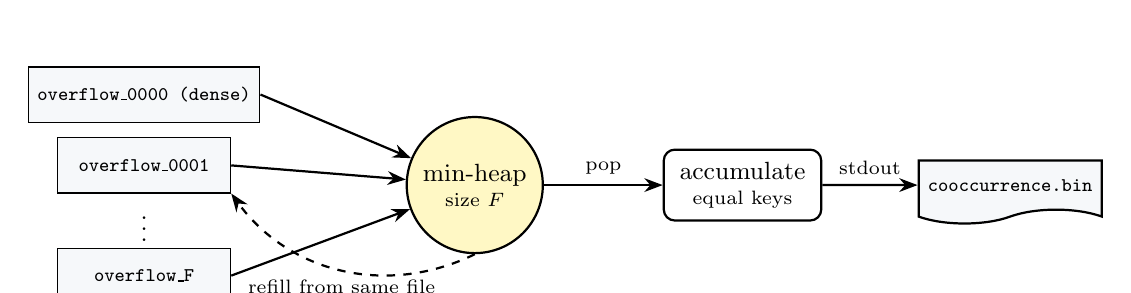
\begin{tikzpicture}[font=\small,
  f/.style={draw,fill=fileC,minimum width=22mm,minimum height=7mm,font=\ttfamily\scriptsize},
  arr/.style={-{Stealth},thick}]
\node[f] (f0) at (0,0) {overflow\_0000 (dense)};
\node[f] (f1) at (0,-0.9) {overflow\_0001};
\node at (0,-1.6) {$\vdots$};
\node[f] (fn) at (0,-2.3) {overflow\_F};
\node[draw,circle,thick,fill=stageB,minimum size=16mm,align=center] (h) at (4.2,-1.15) {min-heap\\[-2pt]\scriptsize size $F$};
\node[draw,rounded corners,thick,minimum width=20mm,minimum height=9mm,align=center] (acc) at (7.6,-1.15) {accumulate\\[-2pt]\scriptsize equal keys};
\node[draw,shape=tape,tape bend top=none,thick,fill=fileC,minimum width=22mm,minimum height=8mm,font=\ttfamily\scriptsize] (out) at (11,-1.15) {cooccurrence.bin};
\foreach \n in {f0,f1,fn} \draw[arr] (\n.east) -- (h);
\draw[arr] (h) -- node[above,font=\scriptsize]{pop} (acc);
\draw[arr] (acc) -- node[above,font=\scriptsize]{stdout} (out);
\draw[arr,dashed] (h.south) to[bend left=40] node[below,font=\scriptsize]{refill from same file} (f1.south east);
\end{tikzpicture}
\caption{Final phase of \texttt{cooccur}: an $F$-way merge that also sums duplicates.}
\end{figure}

\subsection{Choosing \texttt{max\_product} from \opt{memory}}
\label{sec:maxproduct}

\fn{main} turns a memory budget $M$ in gigabytes (GB) into the two buffer sizes:
\[
  R = \frac{0.85\,M\cdot 2^{30}}{\texttt{sizeof(CREC)}},\qquad
  \texttt{overflow\_length} = R/6,
\]
and solves for $P=\texttt{max\_product}$ by fixed-point iteration:
\[
  P\,(\ln P + 0.1544313298) = R.
\]
Where does the constant come from? The number of dense cells is about the number of
integer pairs with $a\,b\le P$, which is $\sum_{k\le P} d(k)$, the divisor summatory
function. Dirichlet's estimate gives $\sum_{k\le P} d(k)\approx P\ln P + (2\gamma-1)P$,
and $2\gamma-1 = 0.15443\ldots$ ($\gamma$ = Euler--Mascheroni). The heuristic therefore
sizes the hyperbolic region of Figure~\ref{fig:hyperbola} to use about 85\% of the
budget, leaving about 1/6 for the overflow buffer. Because cells are divided by
\texttt{sizeof(CREC)}=16 while dense cells are 8-byte \texttt{double}s, the estimate is
conservative. Use \opt{max-product} and \opt{overflow-length} to override it.

\begin{insight}
If you give \texttt{cooccur} more memory, more pairs go to the fast dense path, fewer temp
files are written, and the merge has a smaller fan-in. The output is identical either way.
Only speed and disk use change.
\end{insight}

\section{Stage 3 --- \texttt{shuffle}}

\begin{codeloc}
\file{src/shuffle.c}: \fn{shuffle\_by\_chunks}, \fn{shuffle\_merge}, \fn{shuffle}
(Fisher--Yates), \fn{rand\_long}.
\end{codeloc}

\paragraph{Why shuffle at all?} \file{cooccurrence.bin} is sorted by $w_1$. Training on it
in that order would apply thousands of consecutive updates to the same row $\wv_1$, then
$\wv_2$, and so on. That is very biased SGD. It also defeats Hogwild parallelism
(Section~\ref{sec:hogwild}), because neighbouring records, and records at the same offset
in different threads' slices, would share rows.

\paragraph{Algorithm (two-pass, out-of-core).}
\begin{enumerate}[nosep]
  \item \textbf{Chunk shuffle.} Read up to \texttt{array\_size} records
        ($0.95\,M\cdot2^{30}/16$ by default), Fisher--Yates shuffle them in memory, and write
        \file{temp\_shuffle\_NNNN.bin}. Repeat until EOF.
  \item \textbf{Interleaving merge.} Repeatedly read about \texttt{array\_size}/$F$ records
        from \emph{each} temp file into one buffer, shuffle the buffer, and write it to
        \texttt{stdout}.
\end{enumerate}
This is not a perfectly uniform permutation (the code says ``good enough''), but every
output window mixes records from every part of the input. \fn{rand\_long} combines two
\fn{rand} calls and uses rejection sampling to avoid modulo bias. \opt{seed} makes the
result reproducible; without it the seed is \texttt{time(0)}.

If the input fits in one chunk ($F=1$), the result is a single uniform Fisher--Yates
permutation followed by a second shuffle.

\section{Stage 4 --- \texttt{glove}, the trainer}

\begin{codeloc}
\file{src/glove.c}: \fn{initialize\_parameters}, \fn{glove\_thread} (the inner loop),
\fn{train\_glove} (epoch driver), \fn{save\_params} (output), \fn{main} (command-line parsing).
\end{codeloc}

\subsection{Parameter memory layout}

All parameters live in one contiguous, 128-byte-aligned array \texttt{W} of
$2V(d+1)$ doubles. A parallel array \texttt{gradsq} of the same shape holds the AdaGrad
accumulators.

\begin{figure}[h]
\centering
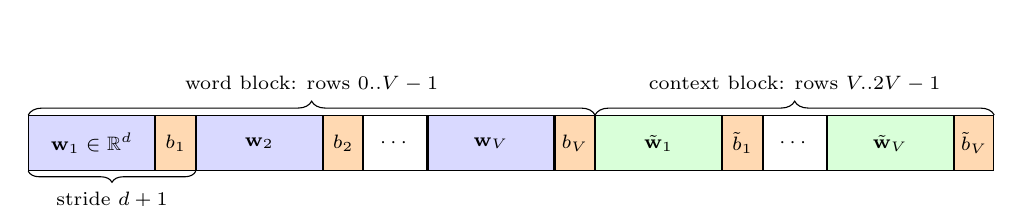
\begin{tikzpicture}[font=\scriptsize,
  c/.style={draw,minimum height=7mm,inner sep=1pt,anchor=west},
  v/.style={c,fill=blue!15,minimum width=16mm},
  b/.style={c,fill=orange!30,minimum width=5mm},
  cv/.style={c,fill=green!15,minimum width=16mm}]
\node[v]  (w1) at (0,0) {$\wv_1\in\R^d$};
\node[b]  (b1) at (w1.east) {$b_1$};
\node[v]  (w2) at (b1.east) {$\wv_2$};
\node[b]  (b2) at (w2.east) {$b_2$};
\node[c,minimum width=8mm] (dots1) at (b2.east) {$\cdots$};
\node[v]  (wV) at (dots1.east) {$\wv_V$};
\node[b]  (bV) at (wV.east) {$b_V$};
\node[cv] (c1) at (bV.east) {$\cv_1$};
\node[b]  (cb1) at (c1.east) {$\tilde b_1$};
\node[c,minimum width=8mm] (dots2) at (cb1.east) {$\cdots$};
\node[cv] (cV) at (dots2.east) {$\cv_V$};
\node[b]  (cbV) at (cV.east) {$\tilde b_V$};
\draw[decorate,decoration={brace,amplitude=5pt}] (w1.north west) -- node[above=5pt]{word block: rows $0..V-1$} (bV.north east);
\draw[decorate,decoration={brace,amplitude=5pt}] (c1.north west) -- node[above=5pt]{context block: rows $V..2V-1$} (cbV.north east);
\draw[decorate,decoration={brace,mirror,amplitude=4pt}] (w1.south west) -- node[below=4pt]{stride $d+1$} (b1.south east);
\end{tikzpicture}
\caption{Layout of \texttt{W} (and \texttt{gradsq}). For a record $(i,j)$ the trainer
computes \texttt{l1}$=(i-1)(d+1)$ and \texttt{l2}$=(j-1+V)(d+1)$. The bias sits at offset $d$
inside each row, so a vector and its bias share cache lines.}
\label{fig:layout}
\end{figure}

\paragraph{Initialisation.} $W_{k}\sim\mathcal U(-0.5,0.5)/d$ for every entry, biases
included, and $\texttt{gradsq}_k=1$. Alternatively, both arrays can be loaded from binary
checkpoints (\opt{load-init-param}, \opt{load-init-gradsq}).

\subsection{The inner loop}

\begin{lstlisting}[caption={Core of \fn{glove\_thread}, lightly condensed.},label=lst:inner]
for each CREC cr in my slice of the file:
    l1 = (cr.word1 - 1) * (d+1);                 // word row
    l2 = (cr.word2 - 1 + V) * (d+1);             // context row
    diff  = dot(W+l1, W+l2, d) + W[l1+d] + W[l2+d] - log(cr.val);
    fdiff = (cr.val > x_max) ? diff : pow(cr.val/x_max, alpha) * diff;
    if (isnan/isinf(diff or fdiff)) continue;
    cost[id] += 0.5 * fdiff * diff;

    for b in 0..d-1:                              // vectors: AdaGrad + clipping
        t1 = clip(fdiff * W[l2+b], +-grad_clip) * eta;   // grad wrt w_i
        t2 = clip(fdiff * W[l1+b], +-grad_clip) * eta;   // grad wrt w~_j
        u1[b] = t1 / sqrt(gradsq[l1+b]);   gradsq[l1+b] += t1*t1;
        u2[b] = t2 / sqrt(gradsq[l2+b]);   gradsq[l2+b] += t2*t2;
    if (sum(u1), sum(u2) finite) { W[l1+b] -= u1[b]; W[l2+b] -= u2[b]; }

    W[l1+d] -= fdiff / sqrt(gradsq[l1+d]);         // biases: AdaGrad, no eta
    W[l2+d] -= fdiff / sqrt(gradsq[l2+d]);
    gradsq[l1+d] += fdiff*fdiff;  gradsq[l2+d] += fdiff*fdiff;
\end{lstlisting}

Written as math, for vector component $k$:
\[
  u = \eta\cdot\operatorname{clip}(g_k),\qquad
  w_k \leftarrow w_k - \frac{u}{\sqrt{G_k}},\qquad
  G_k \leftarrow G_k + u^2,\qquad G_k^{(0)}=1.
\]
This is AdaGrad with three implementation details worth knowing:
\begin{enumerate}[nosep]
  \item The accumulator stores the \emph{scaled} gradient $(\eta g)^2$, and $G$ starts
        at 1, so the first step has size exactly $\eta\, g$. This is what the comment ``So
        initial value of eta is equal to initial learning rate'' means.
  \item The divisor is the accumulator \emph{before} this step's gradient is added.
  \item Both $u_1$ and $u_2$ are computed from the \emph{old} $\wv_i$ and $\cv_j$ before
        either is written, so the update is a true simultaneous gradient step.
\end{enumerate}

\begin{pitfall}
\textbf{Bias updates do not use $\eta$ and are not clipped}: the step is
$g/\sqrt{G}$ with $G$ accumulating $g^2$. Changing \opt{eta} therefore rescales the vector
learning rate but not the bias learning rate. Also, when the NaN (not-a-number) guard rejects a vector
update, \texttt{gradsq} has already been incremented.
\end{pitfall}

\subsection{Hogwild parallelism}
\label{sec:hogwild}

Each epoch, \fn{train\_glove}:
\begin{enumerate}[nosep]
  \item splits the $N$ records into $T$ contiguous slices of $\lfloor N/T\rfloor$ (the last
        thread also takes the remainder);
  \item starts $T$ POSIX threads (pthreads). Each one opens its \emph{own} \texttt{FILE*}, seeks with
        \fn{fseeko} to $\text{id}\cdot\lfloor N/T\rfloor\cdot16$, and streams its slice;
  \item joins all threads and prints the mean cost $\sum_t\texttt{cost}[t]/N$.
\end{enumerate}

\begin{figure}[h]
\centering
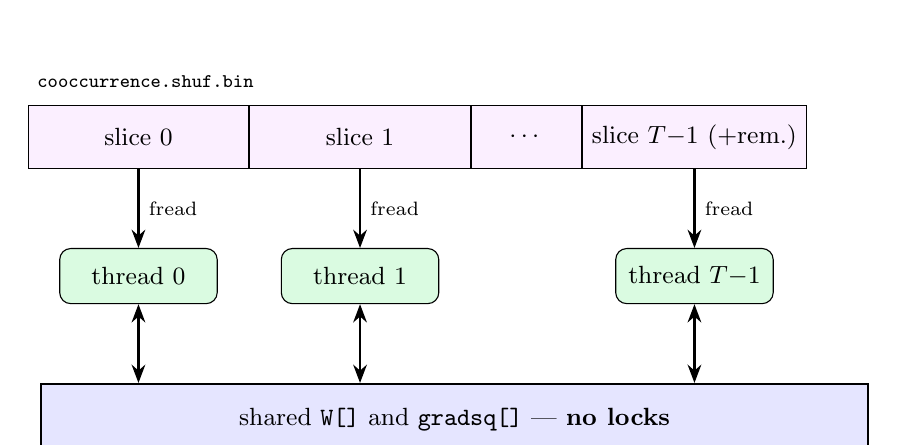
\begin{tikzpicture}[font=\small,
  sl/.style={draw,minimum height=8mm,minimum width=28mm,fill=stageC},
  th/.style={draw,rounded corners,fill=stageD,minimum width=20mm,minimum height=7mm}]
\node[sl] (s0) at (0,0) {slice 0};
\node[sl,right=0 of s0] (s1) {slice 1};
\node[sl,right=0 of s1,minimum width=14mm] (sd) {$\cdots$};
\node[sl,right=0 of sd] (s3) {slice $T{-}1$ (+rem.)};
\node[above=1mm of s0.north west,anchor=south west,font=\ttfamily\scriptsize] {cooccurrence.shuf.bin};
\node[th,below=10mm of s0] (t0) {thread 0};
\node[th,below=10mm of s1] (t1) {thread 1};
\node[th,below=10mm of s3] (t3) {thread $T{-}1$};
\foreach \a/\b in {s0/t0,s1/t1,s3/t3} \draw[-{Stealth},thick] (\a) -- node[right,font=\scriptsize]{fread} (\b);
\node[draw,thick,fill=blue!10,minimum width=105mm,minimum height=9mm,below=10mm of t1.south,xshift=12mm] (W) {shared \texttt{W[]} and \texttt{gradsq[]} --- \textbf{no locks}};
\foreach \t in {t0,t1,t3} \draw[{Stealth}-{Stealth},thick] (\t) -- (\t |- W.north);
\end{tikzpicture}
\caption{One epoch. Threads read disjoint slices of the shuffled file and update shared
parameters without synchronisation (Hogwild!, Recht et al.\ 2011).}
\end{figure}

\textbf{Why lock-free is acceptable.} Each update touches only $2(d+1)$ entries in each of
\texttt{W} and \texttt{gradsq}, out of $2V(d+1)$. After shuffling, two threads rarely touch
the same row at the same moment, and when they do, the race costs at most a lost or stale
update. SGD tolerates that noise. The exception is the most frequent words (ids near 1),
which appear in many records and are contended most. They also receive the most updates,
so they converge anyway.

\begin{pitfall}
Multithreaded training is \textbf{not bit-reproducible}, even with \opt{seed}, because
thread interleaving is nondeterministic. \file{randomization.test.sh} uses
\opt{threads}~1 for this reason.
\end{pitfall}

\subsection{Outputs}
\label{sec:outputs}

\begin{center}
\begin{tabularx}{\linewidth}{lX}
\toprule
\opt{binary} & Files written \\
\midrule
0 (default) & \file{vectors.txt} only \\
1 & \file{vectors.bin} only: the raw \texttt{W} array, $2V(d+1)$ doubles, layout as in
    Figure~\ref{fig:layout}. Reshape to $(2V, d+1)$ to read it. \\
2 & both \\
\bottomrule
\end{tabularx}

\vspace{6pt}
\begin{tabularx}{\linewidth}{lX}
\toprule
\opt{model} & Content of each line of \file{vectors.txt} (\texttt{word v$_1$ \ldots}) \\
\midrule
0 & $[\wv_i, b_i, \cv_i, \tilde b_i]$ --- everything, $2(d+1)$ numbers \\
1 & $\wv_i$ only \\
2 (default) & $\wv_i + \cv_i$ \\
3 & $[\wv_i, \cv_i]$ --- documented in \texttt{--help}, see \S\ref{sec:quirks} \\
\bottomrule
\end{tabularx}
\end{center}

\paragraph{The \texttt{<unk>} vector.} With \texttt{use\_unk\_vec}=1 (hard-coded), the text
output gains a final row \texttt{<unk>} whose vector is the mean of the
$\min(100,V)$ \emph{rarest} words' parameters. Rare words are the best available proxy
for an unseen word. This is why \texttt{<unk>} is banned from the corpus.

\paragraph{Header.} \opt{write-header}~1 prepends \texttt{"V d"}. This makes the file
readable as word2vec text format (for example by gensim), but note that $V$ excludes the
extra \texttt{<unk>} row.

\paragraph{Checkpointing.} \opt{checkpoint-every}~$k$ writes
\file{vectors.NNN.bin} and/or \file{vectors.NNN.txt} every $k$ epochs, and
\opt{save-init-param} writes epoch \texttt{000}. Combined with \opt{gradsq-file} and the
\opt{load-init-param}/\opt{load-init-gradsq} flags, this gives \textbf{exact resume}.
\file{randomization.test.sh} checks that ``2 epochs, then resume for 4'' is byte-identical
to ``6 epochs straight'' when run single-threaded on the same shuffled file.

% =====================================================================
\part{Operating GloVe}
% =====================================================================

\section{Hyper-parameter reference}

\begin{center}
\small
\begin{tabularx}{\linewidth}{llrX}
\toprule
Tool & Flag & Default & Effect / guidance \\
\midrule
vocab\_count & \opt{min-count} & 1 & Drop rare words. 5 for text8, 20 for Wikipedia+Gigaword. \\
             & \opt{max-vocab} & 0 (none) & Hard cap on $V$ (Dolma run used 1.2M). \\
\midrule
cooccur & \opt{window-size} & 15 & Context radius $W$. Smaller windows emphasise syntax, larger ones topical semantics. 10 in the 2024 runs. \\
        & \opt{symmetric} & 1 & 0 = left context only. \\
        & \opt{distance-weighting} & 1 & $1/d$ weighting of pairs. \\
        & \opt{memory} & 3 (help says 4) & Soft budget in GB (see \S\ref{sec:maxproduct}). \\
        & \opt{max-product}, \opt{overflow-length} & auto & Manual overrides. \\
        & \opt{overflow-file} & overflow & Temp file prefix. Put it on fast disk. \\
\midrule
shuffle & \opt{memory} & 2 (help says 4) & Chunk size budget. \\
        & \opt{seed} & time & Reproducible shuffles. \\
        & \opt{temp-file} & temp\_shuffle & Temp file prefix. \\
\midrule
glove & \opt{vector-size} & 50 & $d$. \\
      & \opt{iter} & 25 & Epochs. 50--100 for large corpora. \\
      & \opt{eta} & 0.05 & Initial AdaGrad rate (vectors only). \\
      & \opt{alpha} & 0.75 & Exponent in $f$. \\
      & \opt{x-max} & 100 & Cutoff in $f$. Use about 10 for small corpora. \\
      & \opt{grad-clip} & 100 & Per-component gradient clip. \\
      & \opt{threads} & 8 & Hogwild workers. \\
      & \opt{binary}, \opt{model} & 0, 2 & Output format (see \S\ref{sec:outputs}). \\
      & \opt{seed} & time & Parameter initialisation. \\
\bottomrule
\end{tabularx}
\end{center}

\section{Resource sizing}

\begin{itemize}
  \item \textbf{Trainer RAM} (random-access memory) $\approx 2\times 2V(d+1)\times 8$ bytes (\texttt{W} +
        \texttt{gradsq}). Example: $V=400\text{k}$, $d=300$:
        $2\times 2\cdot400{,}000\cdot301\cdot8 \approx 3.9$ GB.
  \item \textbf{Co-occurrence file} $=16\times\text{nnz}(X)$ bytes. The shuffled copy is
        the same size, and \texttt{shuffle} needs a third copy of temp space while it
        runs, so plan disk for about $3\times$.
  \item \textbf{Epoch cost} $=O(\text{nnz}(X)\cdot d)$, independent of corpus length. The
        paper argues that, under a power-law model of counts, $\text{nnz}(X)$ grows
        sub-linearly in corpus size $|C|$ (about $|C|^{0.8}$ for their data). This is the
        main efficiency argument against window-scanning methods.
  \item \textbf{I/O (input/output) pattern}: every stage streams sequentially. \texttt{glove} re-reads the
        whole shuffled file every epoch, $T$ streams in parallel, so page-cache or solid-state drive (SSD)
        throughput matters.
\end{itemize}

\section{Evaluation}

\file{eval/python/evaluate.py} runs the Google analogy benchmark:
\begin{enumerate}[nosep]
  \item Load \file{vocab.txt} and \file{vectors.txt} (skipping \texttt{<unk>}), then
        L2-normalise every row.
  \item For each question $a:b::c:?$, compute $\mathbf q = \hat\wv_b - \hat\wv_a + \hat\wv_c$
        and predict $\arg\max_x \hat\wv_x^\top\mathbf q$, excluding $a,b,c$. Questions are
        processed in batches of 100 as one matrix product.
  \item Report top-1 accuracy per file and aggregated: the first five files are
        \emph{semantic} (capitals, currency, family, \ldots) and the other nine are
        \emph{syntactic} (plurals, tenses, \ldots). Questions with out-of-vocabulary
        words are skipped, and ``Questions seen/total'' reports coverage.
\end{enumerate}
\file{distance.py} gives interactive nearest neighbours and \file{word\_analogy.py} gives
interactive analogies. The MATLAB and Octave directories implement the same benchmark.

\section{Reproducibility}

\begin{center}
\begin{tabularx}{\linewidth}{lXl}
\toprule
Stage & Source of randomness & Control \\
\midrule
vocab\_count & none; ties are broken alphabetically (\opt{max-vocab} truncation depends on \fn{qsort} order) & --- \\
cooccur & none & --- \\
shuffle & \fn{rand} & \opt{seed} \\
glove & init \fn{rand}; thread scheduling & \opt{seed} + \opt{threads} 1 \\
\bottomrule
\end{tabularx}
\end{center}

\section{Known quirks found while reading the code}
\label{sec:quirks}

These are observations from the current source, not documented behaviour.

\begin{enumerate}
  \item \textbf{\opt{model}~3 is unreachable.} \fn{main} in \file{glove.c} runs
        \texttt{if (model != 0 \&\& model != 1) model = 2;}, so a requested 3 is silently
        changed to 2, even though \fn{save\_params} has a branch for 3 and \texttt{--help}
        documents it.
  \item \textbf{Bias learning rate ignores \opt{eta}} and is not clipped (see
        Listing~\ref{lst:inner}).
  \item \textbf{Default/help mismatches.} \texttt{cooccur}'s \texttt{memory\_limit}
        defaults to 3 GB and \texttt{shuffle}'s to 2 GB, while both help texts say 4.0.
        The \texttt{-memory} flag overrides both.
  \item \textbf{Help invocation differs by tool.} \texttt{cooccur} and \texttt{glove} print
        help when given no arguments, while \texttt{vocab\_count} and \texttt{shuffle}
        need \texttt{-h}, because they read \texttt{stdin} by default.
  \item \textbf{\texttt{-Ofast} breaks NaN guards.} As the \file{Makefile} warns,
        \texttt{-ffast-math} assumes finite values, so \fn{isnan}/\fn{isinf} checks are
        optimised away. The default build uses \texttt{-O3}.
  \item \textbf{\texttt{calloc(num, sizeof(FILE))}} in \fn{merge\_files} and
        \fn{shuffle\_merge} allocates \texttt{sizeof(FILE)} instead of
        \texttt{sizeof(FILE*)} per slot. This over-allocates but is otherwise harmless.
\end{enumerate}

\section{Mental model: one-paragraph summary}

\begin{tcolorbox}[colback=gray!4,colframe=gray!50!black,title=\textbf{GloVe in one paragraph}]
Count how often every pair of words appears near each other, discounting by distance and
never crossing a newline. Do this once, using a dense array for the Zipf-head pairs and
sorted spill files for the long tail, then merge everything into one sorted list of
non-zero $(i,j,X_{ij})$ records. Shuffle that list. Then, for 15--100 passes, let several
threads stream disjoint parts of it and, without locking, nudge
$\wv_i^\top\cv_j+b_i+\tilde b_j$ towards $\log X_{ij}$, weighting each nudge by
$f(X_{ij})$ and scaling it per coordinate with AdaGrad. At the end, write
$\wv_i+\cv_i$ for each word, plus an \texttt{<unk>} vector averaged from the rarest words.
\end{tcolorbox}

\section*{References}
\addcontentsline{toc}{section}{References}
\begin{enumerate}[label={[\arabic*]},leftmargin=2em]
  \item J.~Pennington, R.~Socher, C.~D.~Manning. \emph{GloVe: Global Vectors for Word
        Representation}. Conference on Empirical Methods in Natural Language Processing (EMNLP) 2014. \url{https://nlp.stanford.edu/pubs/glove.pdf}
  \item T.~Mikolov et al. \emph{Distributed Representations of Words and Phrases and their
        Compositionality}. Conference on Neural Information Processing Systems (NeurIPS) 2013.
  \item J.~Duchi, E.~Hazan, Y.~Singer. \emph{Adaptive Subgradient Methods for Online
        Learning and Stochastic Optimization} (AdaGrad). Journal of Machine Learning Research (JMLR) 2011.
  \item B.~Recht, C.~Re, S.~Wright, F.~Niu. \emph{Hogwild!: A Lock-Free Approach to
        Parallelizing Stochastic Gradient Descent}. NeurIPS 2011.
  \item Project page and pre-trained vectors: \url{https://nlp.stanford.edu/projects/glove/}
\end{enumerate}

\end{document}
